\chapter{Technical design} \label{chap:tech_design}
% describe specific implementation details
\section{Quantum sensing setup}
\section{Photodetection PCB}
As an integral part of the sensing setup, the photodetection PCB needs a lot of attention. Good amplification is crucial to increasing the \gls{snr} of the quantum setup. Based on the design ideas presented in the functional design (see Chapter \ref{chap:photodetection_design}), the photodetection circuit can be drawn up. Simulating every iteration is necessary to ensure the calculations are correct 

\subsection{First iteration}
As previously mentioned, the first iteration of the PCB uses component values provided by the client. Figure \ref{fig:photodetecog} shows the LTSpice design. $C_1$ and $R_2$, as well as the current source $I_1$ are used to simulate the behavior of a photodiode.

\begin{figure} [ht]
	\centering
	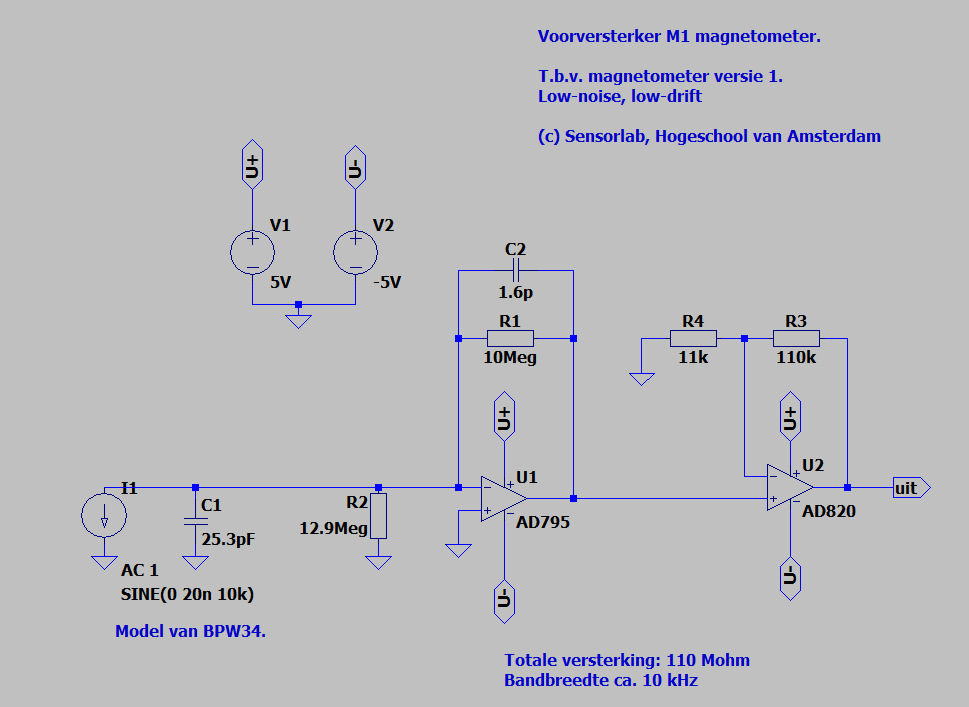
\includegraphics[width=0.7\linewidth]{img/photodetec_og}
	\caption{Provided photodetector design}
	\label{fig:photodetecog}
\end{figure}


\subsubsection{Simulation}
Tina-TI was used to simulate and visualize the DC gain and frequency response of the system, as seen in Figure \ref{fig:tina2probes}. The signals $V_{ot}$ and $V_{out}$ correspond to the output of the transimpedance and non-inverting amplification stage respectively. The AC plot (Figure \ref{fig:tinaac2probes}) shows the cutoff, at \num{10,77} \unit{\kilo \hertz}, and the gain inside the gain bandwidth, which is \num{160,82} \unit{\decibel}. The DC plot (Figure \ref{fig:tinadc2probes}) shows the voltage with respect to the current and demonstrates the linearity of the system in the range of \numrange{0}{46,31} \unit{\nano \second}. After $V_{out}$ reaches \num{5} \unit{V}, the output remains fixed, because it cannot exceed the voltage provided to the amplifier. 

\begin{figure}[ht]
	\centering
	\begin{subfigure}[1a]{.49\linewidth}
		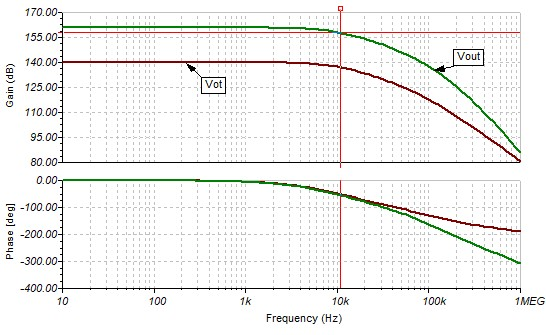
\includegraphics[width=\linewidth]{img/tina_AC_2probes}
		\caption{Frequency response}
		\label{fig:tinaac2probes}
	\end{subfigure}
	\hfill
	\begin{subfigure}[1b]{.49\linewidth}
		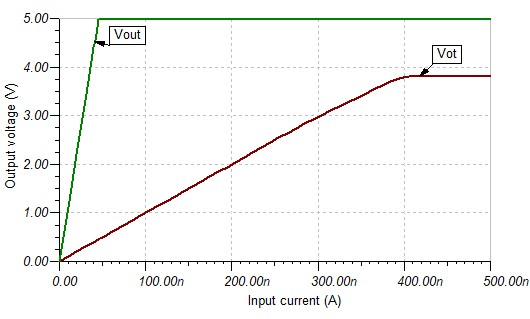
\includegraphics[width=\linewidth]{img/tina_DC_2probes}
		\caption{DC gain}
		\label{fig:tinadc2probes}
	\end{subfigure}
	\caption{Simulation of the first iteration of the photodetector}
	\label{fig:tina2probes}
\end{figure}


\subsubsection{Implementation} 

\begin{figure}[ht]
	\centering
	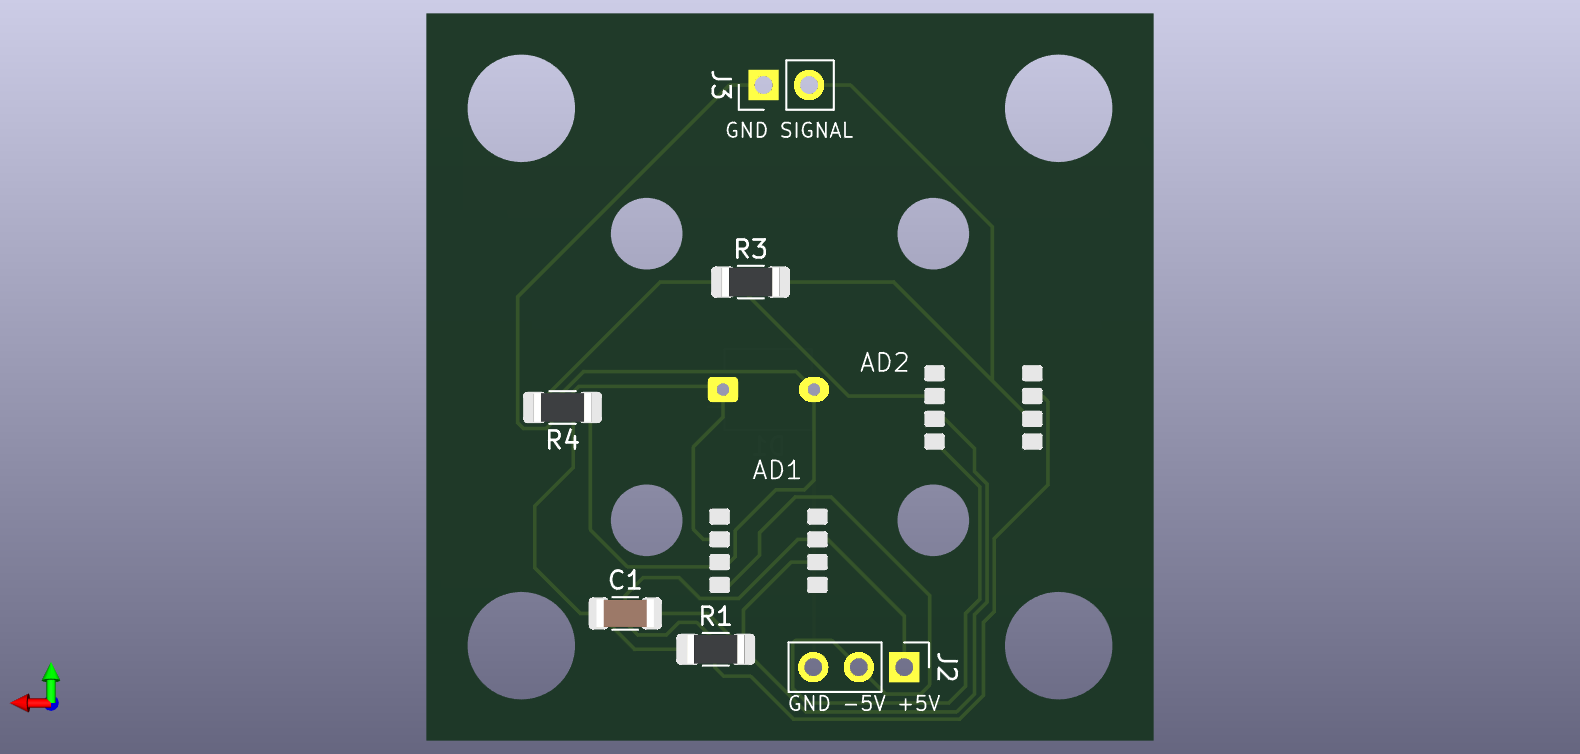
\includegraphics[width=0.7\linewidth]{img/photodetec_og_pcb}
	\caption{First iteration of the photodetection PCB}
	\label{fig:photodetecogpcb}
\end{figure}


\section{OLIA implementation}
